\chapter{METODOLOGÍA DE LA INVESTIGACIÓN}
\section{Diseño de la investigación}
En esta sección del documento se explicará cual es el diseño, el tipo y el enfoque del trabajo de
investigación, así como también la población y la muestra. 
%Para finalizar se explicará el
%proceso de aplicación de las redes neuronales convolucionales.
\subsection{Diseño no experimental}
El diseño es no experimental transversal, ya que las variables no serán manipuladas y serán analizadas tal como se encuentran. Es decir, tanto los datos visuales de las hojas de papa peruana afectadas por la enfermedad 'Rancha' (Phytophthora infestans) como las técnicas de visión computacional serán utilizados sin modificar ningún aspecto de las condiciones naturales. El objetivo es aplicar técnicas de visión computacional para clasificar tempranamente la presencia de la enfermedad en las hojas de papa. La recolección de datos se llevará a cabo en un periodo de tiempo específico, sin intervenir en el desarrollo natural de la enfermedad en las plantas

\subsection{Tipo explicativo}
El alcance de esta investigación es explicativo, ya que se enfoca en construir un modelo de visión computacional para la detección temprana de la enfermedad 'Rancha' (Phytophthora infestans) a partir de imágenes de hojas de papa. Esto busca entender cómo identificar si una hoja de papa está afectada por el tizón tardío, estableciendo así una relación de causa y efecto. En otras palabras, al identificar un patrón específico en las hojas de papa con Rancha, se podrá determinar si están afectadas por la patología.

\subsection{Enfoque cuantitativo}
El enfoque de esta investigación es cuantitativo, dado que se emplearán técnicas de visión computacional, las cuales implican procesar datos de imagen en valores numéricos (vectores de características). Posteriormente, se usarán técnicas estadísticas para analizar estos datos y determinar la presencia de la enfermedad 'Rancha' (Phytophthora infestans) en las hojas de papa peruana.

\section{Población y Muestra }

\begin{table}[H]
	\centering
	\caption{Poblacion y muestra }
	\label{tabla-2x4}
	\begin{tabular}{|p{3cm}|p{9cm}|}
		\hline
		Poblacion &  La población fueron todas las imágenes de hojas de papa infestadas con Tizón tardío hojas de papa sanas.  \\ \hline
		Muestra &  La muestra se extrajo un conjunto de imágenes de los dataset Plant Diseases Training Dataset, el cual es una recopilación de otras agrupaciones de datos como PlantVillage, Potato Leaf Disease, Cassava Leaf Disease Dataset, etc. Se cuenta con 1777 imágenes de hojas de papa etiquetadas como sanas y 2020 como infestada con Tizón tardío. Adicionalmente, cabe mencionar, que para el propósito de esta investigación se utilizará 80\% del conjunto de imágenes total para Training y 20\% para el Testing de los modelos correspondientes.\\ \hline
		Unidad de análisis &  En este caso, la unidad de análisis es cada imagen individual de hojas de papa, tanto sanas como infestadas con Tizón tardío. \\ \hline
		Variable y tipo de analisis & Variable cuantitativa y discreta, debido a que el presente trabajo de
		investigación está centrado en variables numéricas y la precisión o
		exactitud. \\ \hline
	\end{tabular}
\end{table}


\begin{figure}[H]
	\begin{center}
		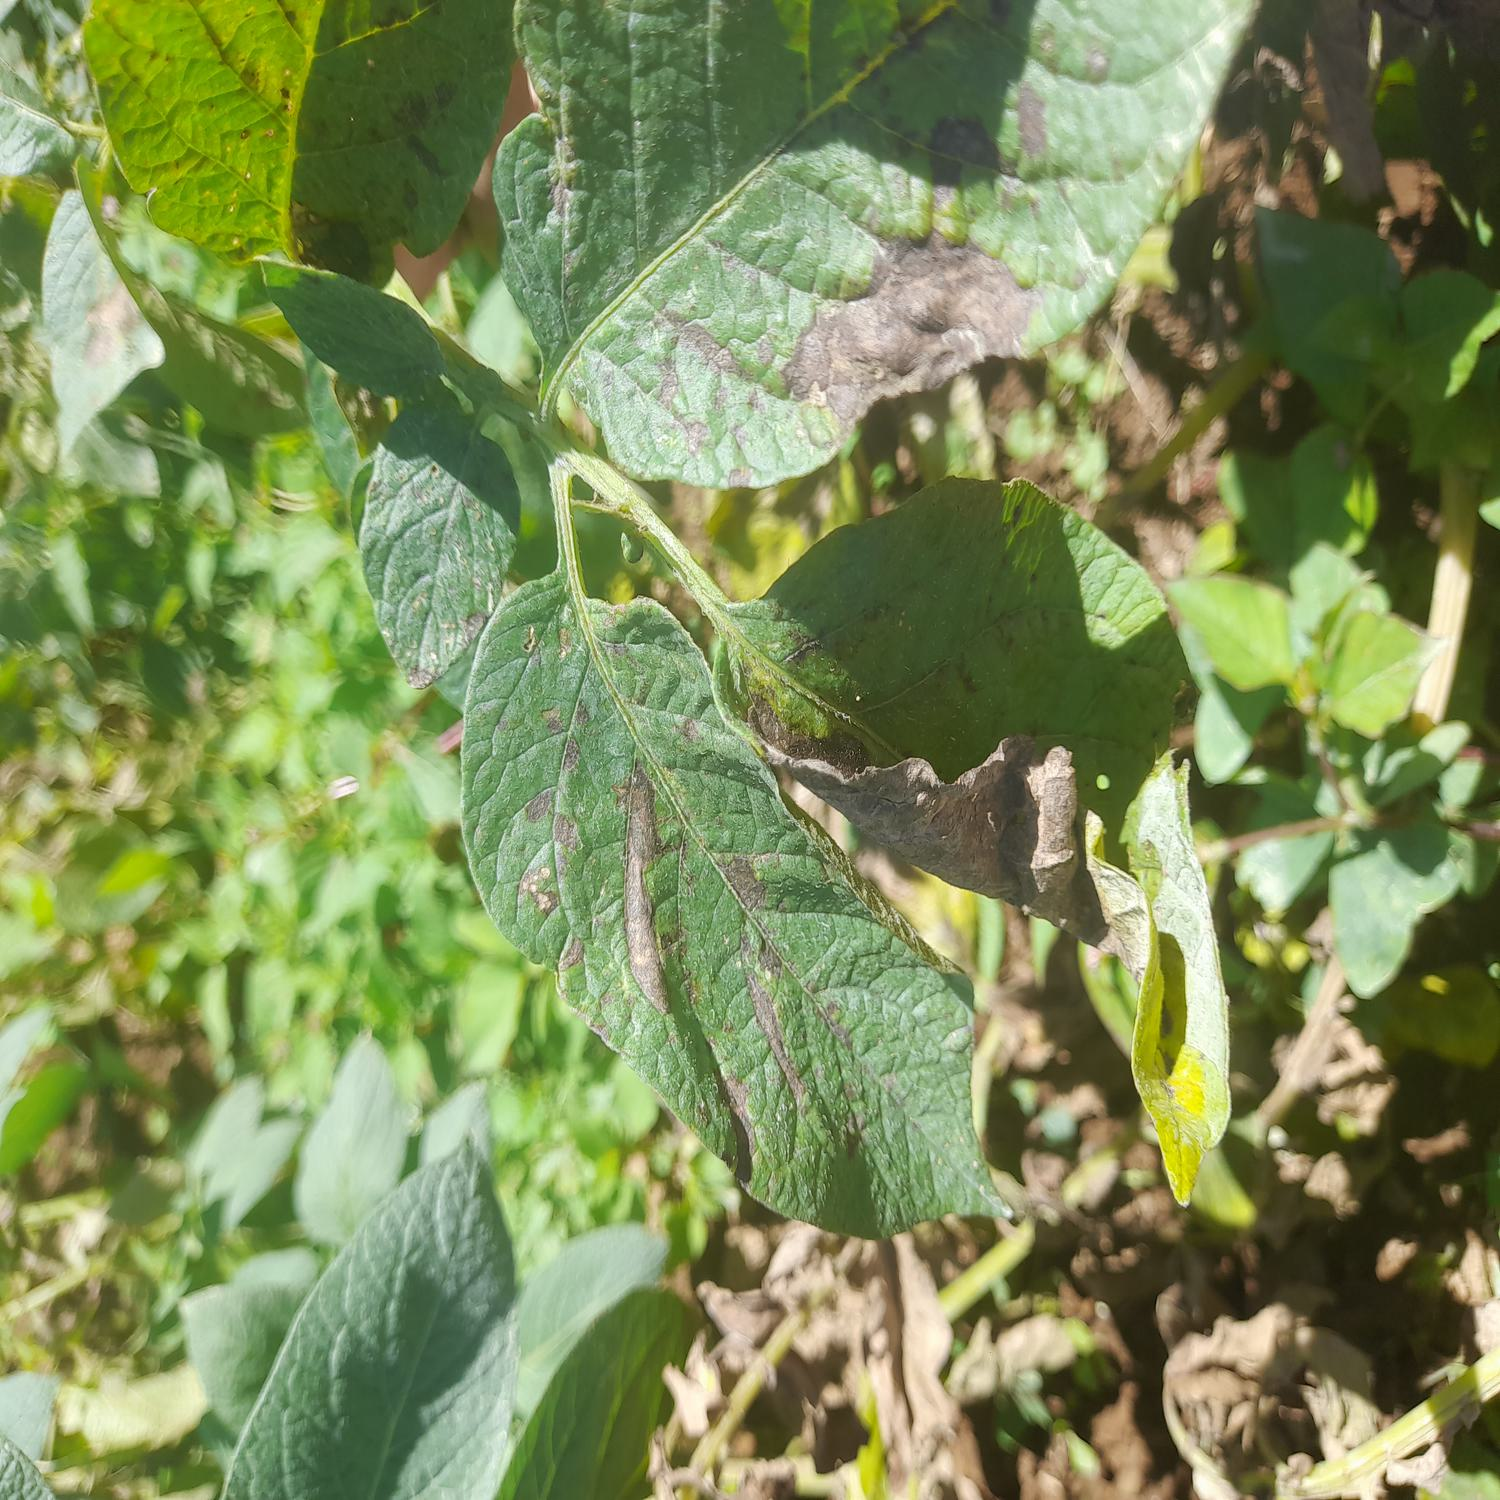
\includegraphics[width=0.8\textwidth]{3/figures/img.jpg}
		\caption{Hoja de papa infestada con Tizón tardío}
		\label{fig1}
	\end{center}
	
\end{figure}

\section{Operacionalizacion de Variables}
% Please add the following required packages to your document preamble:
% \usepackage{multirow}
\begin{table}[H]
	\begin{tabular}{lll}
		\hline
		\multicolumn{3}{l}{Definción de Variables}                                                                                                                                                                                                                                                                                                                                                                                                                                                             \\ \hline
		\multicolumn{1}{|l|}{VARIABLE Y DEFINICIÓN}                                                                                                                                                                                                       & \multicolumn{1}{l|}{INDICADOR}                                                                                 & \multicolumn{1}{l|}{FÓRMULA DE INDICADOR}                                                                                         \\ \hline
		\multicolumn{1}{|l|}{\begin{tabular}[c]{@{}l@{}}TIZON TARDIO \\ Enfermedad causada por \\ un hongo que afecta a los \\ tomates y papas, \\ provocando manchas oscuras \\ en las hojas y frutos\end{tabular}}                                      & \multicolumn{1}{l|}{Hoja de papa}                                                                              & \multicolumn{1}{c|}{Zona con manchas oscuras en la hoja}                                                                          \\ \hline
		\multicolumn{1}{|l|}{\multirow{5}{*}{\begin{tabular}[c]{@{}l@{}}VISION COMPUTACIONAL\\ Disciplina científica \\ que incluye métodos para \\ adquirir, procesar, analizar y \\ comprender las imágenes \\ del mundo real.\end{tabular}}}           & \multicolumn{1}{l|}{\multirow{3}{*}{Resolución de la imagen}}                                                  & \multicolumn{1}{l|}{\multirow{3}{*}{Cantidad de pixeles en una imagen}}                                                           \\
		\multicolumn{1}{|l|}{}                                                                                                                                                                                                                            & \multicolumn{1}{l|}{}                                                                                          & \multicolumn{1}{l|}{}                                                                                                             \\
		\multicolumn{1}{|l|}{}                                                                                                                                                                                                                            & \multicolumn{1}{l|}{}                                                                                          & \multicolumn{1}{l|}{}                                                                                                             \\ \cline{2-3} 
		\multicolumn{1}{|l|}{}                                                                                                                                                                                                                            & \multicolumn{1}{l|}{\multirow{2}{*}{\begin{tabular}[c]{@{}l@{}}Preprocesamiento \\ de la imagen\end{tabular}}} & \multicolumn{1}{l|}{\multirow{2}{*}{\begin{tabular}[c]{@{}l@{}}Nivel de nitidez, \\ contraste o ruido de la imagen\end{tabular}}} \\
		\multicolumn{1}{|l|}{}                                                                                                                                                                                                                            & \multicolumn{1}{l|}{}                                                                                          & \multicolumn{1}{l|}{}                                                                                                             \\ \hline
		\multicolumn{1}{|l|}{\multirow{9}{*}{\begin{tabular}[c]{@{}l@{}}MODELO DE CLASIFICACIÓN:\\ \\ Modelo con la capacidad de \\ clasificar segun la \\ clase de la variable, \\ evaluado con las metricas\\  mas conocidas y robustas.\end{tabular}}} & \multicolumn{1}{l|}{\multirow{5}{*}{Accuracy}}                                                                 & \multicolumn{1}{l|}{\multirow{5}{*}{\(\frac{TP + TN}{TP + FP + FN + TN}\)}}                                                       \\
		\multicolumn{1}{|l|}{}                                                                                                                                                                                                                            & \multicolumn{1}{l|}{}                                                                                          & \multicolumn{1}{l|}{}                                                                                                             \\
		\multicolumn{1}{|l|}{}                                                                                                                                                                                                                            & \multicolumn{1}{l|}{}                                                                                          & \multicolumn{1}{l|}{}                                                                                                             \\
		\multicolumn{1}{|l|}{}                                                                                                                                                                                                                            & \multicolumn{1}{l|}{}                                                                                          & \multicolumn{1}{l|}{}                                                                                                             \\
		\multicolumn{1}{|l|}{}                                                                                                                                                                                                                            & \multicolumn{1}{l|}{}                                                                                          & \multicolumn{1}{l|}{}                                                                                                             \\ \cline{2-3} 
		\multicolumn{1}{|l|}{}                                                                                                                                                                                                                            & \multicolumn{1}{l|}{\multirow{2}{*}{Precision}}                                                                & \multicolumn{1}{l|}{\multirow{2}{*}{\(\frac{TP}{TP + FP}\)}}                                                                      \\
		\multicolumn{1}{|l|}{}                                                                                                                                                                                                                            & \multicolumn{1}{l|}{}                                                                                          & \multicolumn{1}{l|}{}                                                                                                             \\ \cline{2-3} 
		\multicolumn{1}{|l|}{}                                                                                                                                                                                                                            & \multicolumn{1}{l|}{\multirow{2}{*}{Recall}}                                                                   & \multicolumn{1}{l|}{\multirow{2}{*}{\(\frac{TP}{TP + FN}\)}}                                                                      \\
		\multicolumn{1}{|l|}{}                                                                                                                                                                                                                            & \multicolumn{1}{l|}{}                                                                                          & \multicolumn{1}{l|}{}                                                                                                             \\ \hline
		&                                                                                                                &                                                                                                                                   \\ \hline
	\end{tabular}
\end{table}
\section{Técnicas de recolección de Datos}
En el contexto de una tesis sobre la "Implementación de técnicas de Visión Computacional para la detección temprana de 'Rancha' (Phytophthora infestans) en hojas de papa peruana", la técnica de recolección de datos más importante sería la captura y anotación de imágenes de hojas de papa. 

\subsection{Captura de Imágenes}
Cámaras de Alta Resolución: Utilizar cámaras de alta resolución para capturar imágenes detalladas de las hojas de papa.
Condiciones de Iluminación Controladas: Asegurar que las imágenes se tomen en condiciones de iluminación controladas para evitar sombras y variaciones de color que puedan afectar la precisión de la detección.
Diversidad de Condiciones: Capturar imágenes en diferentes condiciones ambientales (luz solar, sombra, humedad) y etapas de crecimiento de la planta para asegurar que el modelo de visión por computadora sea robusto y generalizable.

\subsection{Anotación de Imágenes}
Etiquetado de Datos: Colaborar con expertos en fitopatología para etiquetar las imágenes, identificando áreas afectadas por la 'Rancha' (Phytophthora infestans).
Software de Anotación: Utilizar herramientas de software de anotación de imágenes que permitan marcar con precisión las áreas afectadas en cada imagen.

\section{Técnicas para el Procesamiento y Análisis de Información}
\subsection{Metodología de la implementación de la solución}
De acuerdo con Szeliski R. (2010), la Visión Computacional se compone de varias etapas que abarcan desde la captura de una imagen hasta su interpretación. Para alcanzar la etapa final, la imagen capturada debe pasar por un proceso que se describirá en detalle en los próximos puntos. La metodología de este trabajo de investigación se ilustra gráficamente en la siguiente Figura.
\begin{figure}[H]
	\begin{center}
		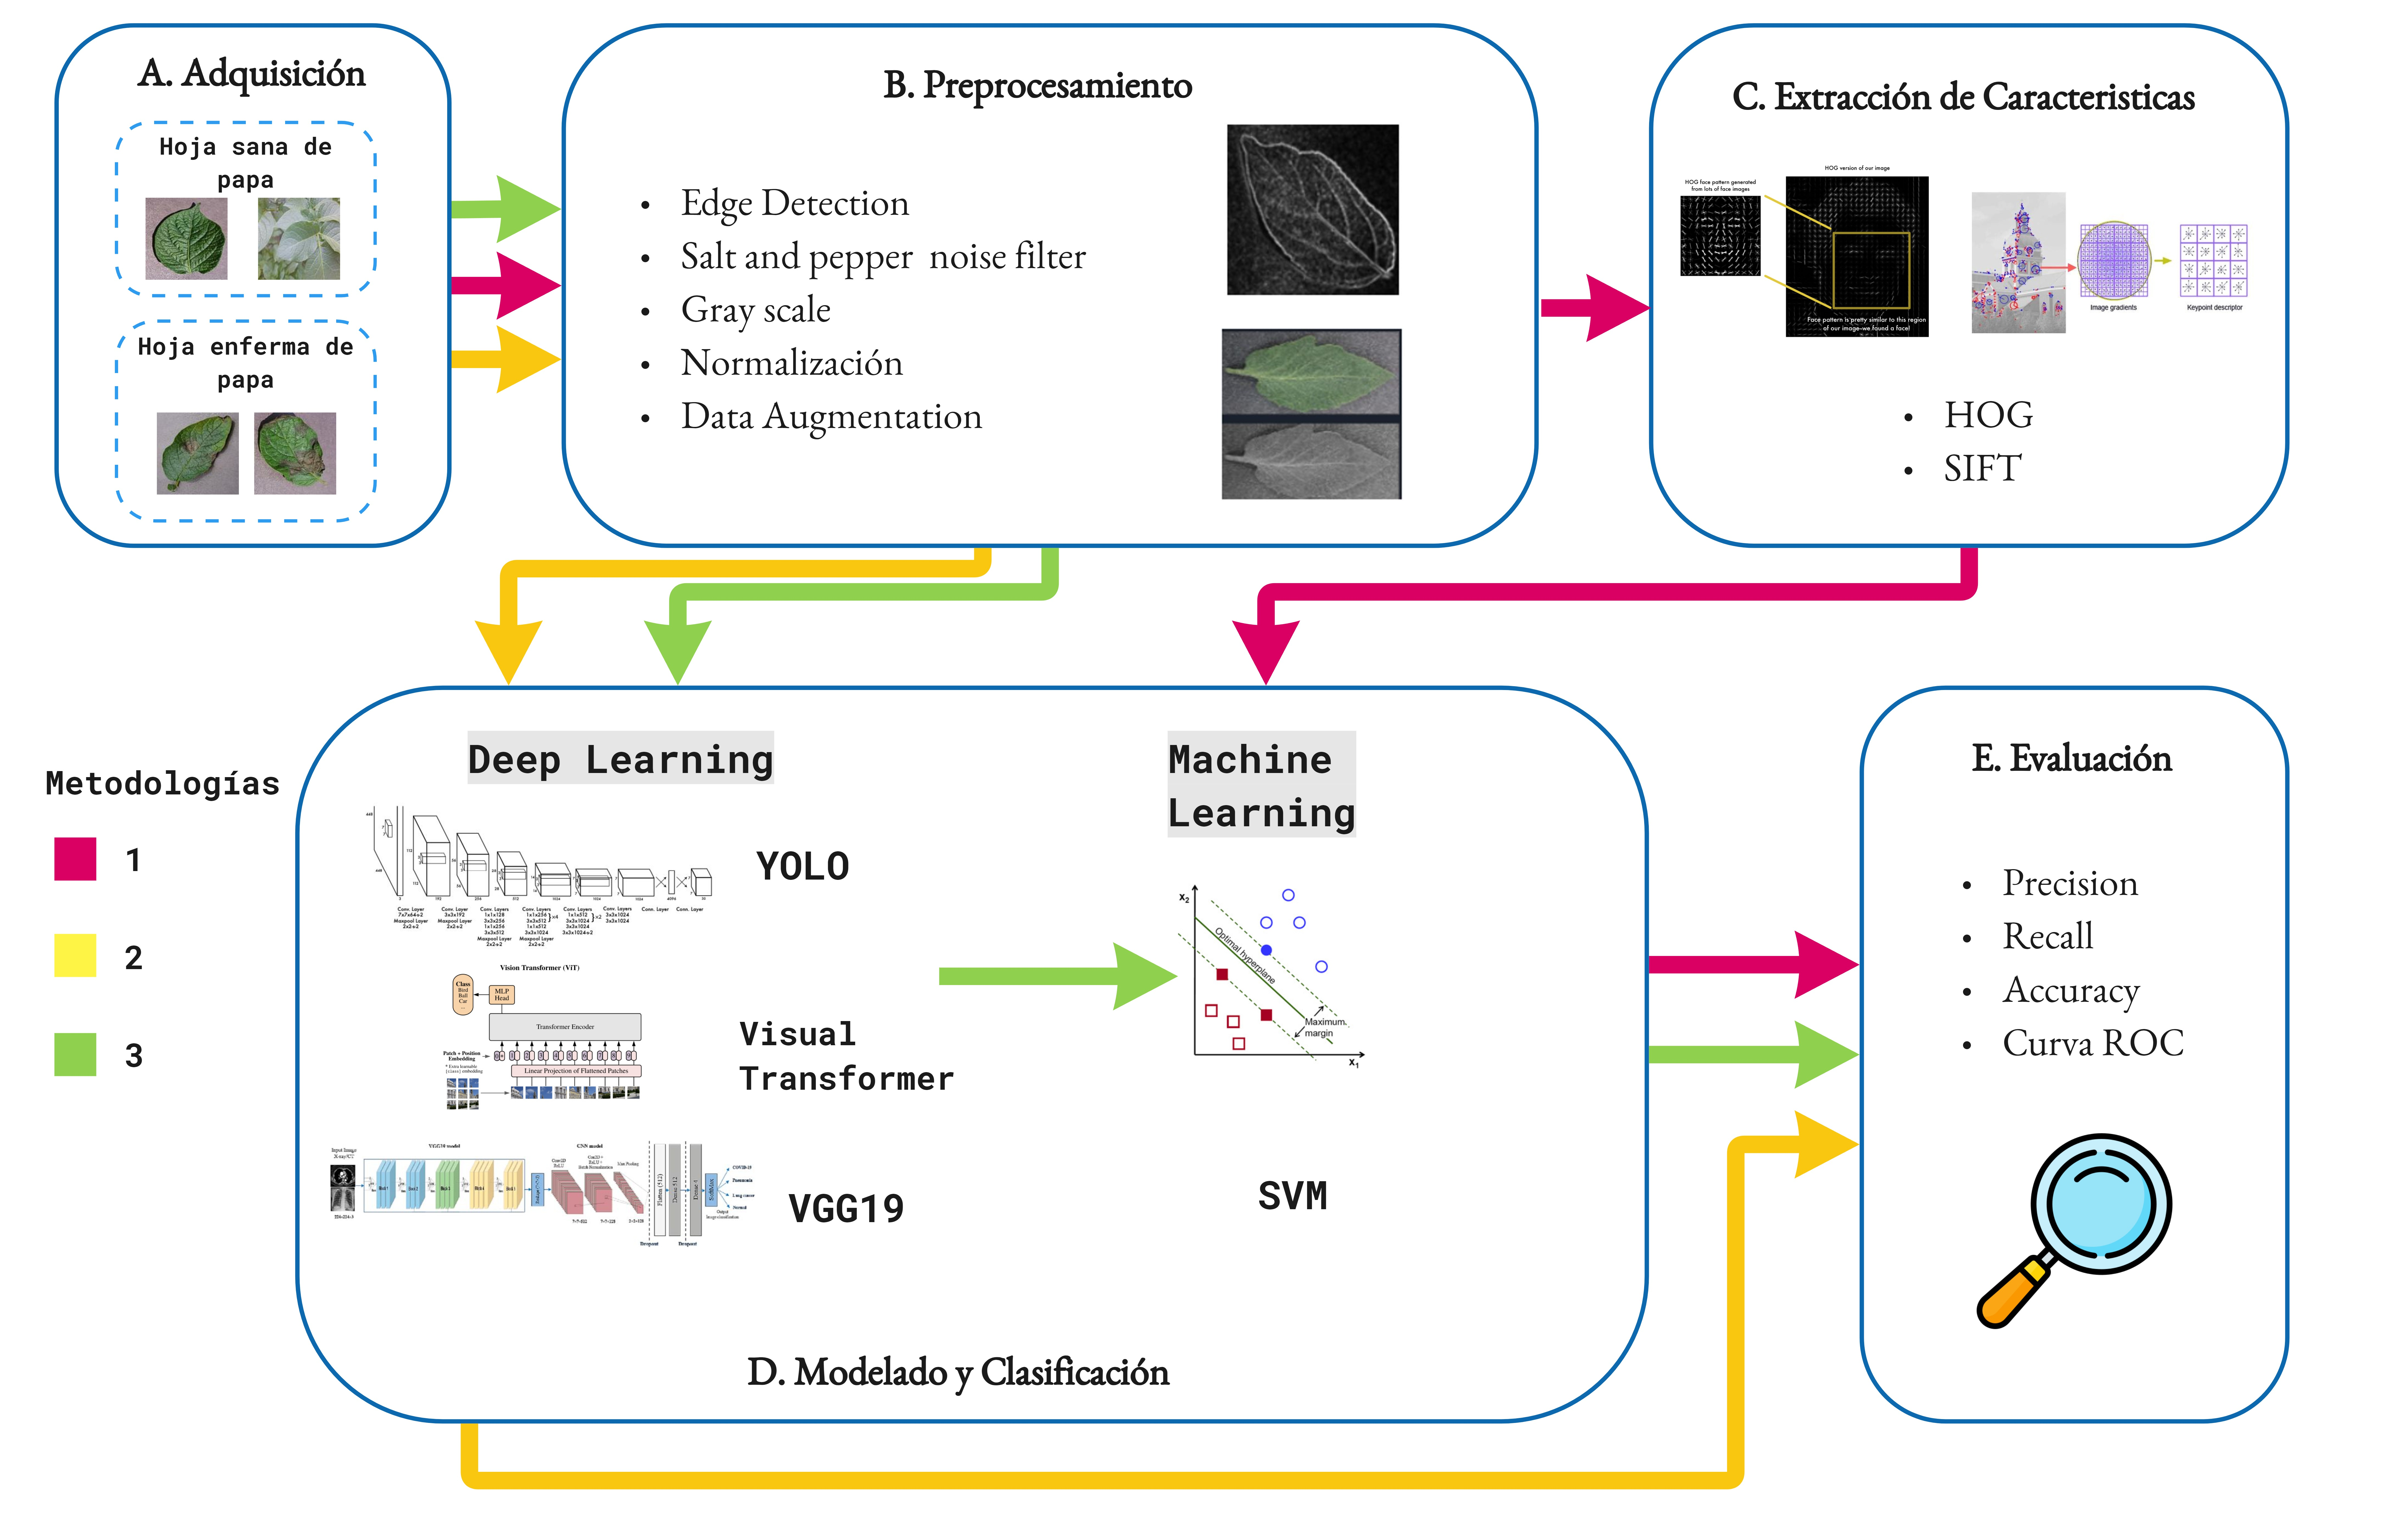
\includegraphics[width=1\textwidth]{3/figures/metodologia.jpg}
		\caption{Metodologia de la Investigacion}
		\label{}
	\end{center}
\end{figure}

\subsection{Metodología para la medición de resultados}
El análisis de los resultados de la implementación se llevó a cabo evaluando la relación entre las variables definidas, con el objetivo de medir la efectividad del modelo de clasificación.

\begin{figure}[H]
	\begin{center}
		
\includegraphics[width=0.8\textwidth]{3/figures/meto2.jpg}
		\caption{Medición de resultados de implementación}
		\label{}
	\end{center}
\end{figure}

Una vez entrenados los modelos de Machine Learning y Deep Learning , se procede a evaluarlos utilizando las siguientes métricas:

Accuracy:
El Accuracy es una métrica que indica la proporción de observaciones correctamente predichas en relación con el total de observaciones. Esta métrica es útil cuando el conjunto de datos tiene una distribución simétrica de falsos positivos y falsos negativos; de lo contrario, puede no ser completamente confiable (Joshi, 2016).

\text{Accuracy} = \(\frac{TP + TN}{TP + FP + FN + TN}\)

Precision:
La Precisión es una medida que indica qué proporción de las predicciones positivas son correctas en relación con el total de predicciones positivas realizadas. Una alta precisión implica una baja tasa de falsos positivos (Joshi, 2016).

\text{Precision} = \(\frac{TP}{TP + FP}\)


Recall:
El Recall es una medida que indica qué proporción de las observaciones positivas reales son identificadas correctamente entre todas las observaciones positivas predichas. (Joshi, 2016)

\text{Recall} = \(\frac{TP}{TP + FN}\)

F1 Score:
El F1 Score es un promedio ponderado de Precision y Recall, lo que significa que considera tanto los falsos positivos como los falsos negativos. Esta métrica es especialmente útil cuando se trabaja con conjuntos de datos desbalanceados, es decir, cuando las observaciones de las clases no están distribuidas de manera uniforme. (Joshi, 2016)

\text{F1 Score} = \(2 \times \frac{TP}{TP + FN}\)

Donde:

TP = True Positives: Son aquellos valores positivos predichos correctamente.

FP = False Positives: Son aquellos valores negativos predichos correctamente.

TN = True Negatives: Son aquellos valores positivos predichos incorrectamente.

FN = False Negatives: Son aquellos valores negativos predichos incorrectamente.
